\documentclass[a4paper]{article}
\usepackage[a4paper,margin=0mm]{geometry}
\usepackage{fontspec}
\usepackage{unicode-math}
\usepackage{tikz}
\usepackage[table]{xcolor}
\usepackage[absolute]{textpos}
\usepackage{enumitem}
\usepackage{array}
\usepackage{multirow}

\setmainfont{Libertinus Serif}
\setsansfont{Libertinus Sans}
\setmathfont{Libertinus Math}
\newfontfamily\trackedsans{Libertinus Sans}[LetterSpace=8.0]

\definecolor{accent}{HTML}{F46530}
\definecolor{badge}{HTML}{FFBDA5}
\definecolor{ink}{HTML}{2A2E30}

\setlength{\TPHorizModule}{1mm}
\setlength{\TPVertModule}{1mm}
\setlength{\parindent}{0pt}
\pagestyle{empty}

\newcommand{\LCOL}{16mm}
\newcommand{\RCOL}{111mm}
\newcommand{\COLW}{83mm}

\newcommand{\topicheader}[2]{%
\begin{textblock*}{194mm}(16mm,10mm)
\begin{tikzpicture}
\node[fill=accent,text=white,font=\sffamily\bfseries\fontsize{13}{13}\selectfont,
      minimum width=9mm,minimum height=9mm,inner sep=0pt] at (4.5mm,-4.5mm) {#1};
\node[font=\sffamily\bfseries\fontsize{15}{16}\selectfont,text=ink,anchor=west] at (12mm,-4.5mm) {#2};
\end{tikzpicture}
\end{textblock*}
\begin{textblock*}{194mm}(16mm,22.5mm)

\begin{tikzpicture}
\fill[accent] (0,0) rectangle (194mm,0.5mm);
\end{tikzpicture}
\end{textblock*}
}

\newcommand{\pagefooter}[1]{%
\begin{textblock*}{194mm}(8mm,286.41mm)
  
\begin{tikzpicture}
    \fill[accent] (0,0) rectangle (194mm,0.6mm);
  \end{tikzpicture}
\end{textblock*}
\begin{textblock*}{63.59mm}(8mm,288.27mm)
  {\sffamily\bfseries\color{accent}\fontsize{13}{16}\selectfont SAT 1200+}
\end{textblock*}
\begin{textblock*}{10mm}(188mm,288.27mm)
  \centering{\sffamily\color{accent}\fontsize{14}{16}\selectfont #1}
\end{textblock*}
}

\newcommand{\colrule}[2]{%
\begin{textblock*}{1mm}(105mm,#1mm)
\begin{tikzpicture}
\draw[black!65,line width=0.5pt] (0,0) -- (0,#2mm);
\end{tikzpicture}
\end{textblock*}
}

\newcommand{\setkicker}[2]{%
{\sffamily\bfseries\fontsize{12}{14}\selectfont #1.}\ {\itshape\fontsize{11}{14}\selectfont\color{black!75} #2}\par\vspace{2mm}%
}

\setlength{\fboxsep}{1.4pt}
\setlength{\fboxrule}{0.5pt}
\newcommand{\pnum}[1]{\fcolorbox{ink}{white}{\sffamily\bfseries\fontsize{8}{8}\selectfont #1}~}

\newcommand{\qrbox}[1]{%
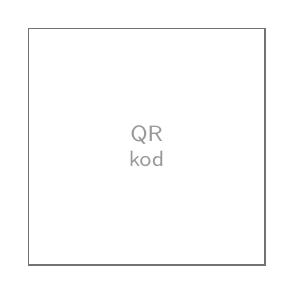
\begin{tikzpicture}
\draw[black!55,line width=0.6pt] (0,0) rectangle (30mm,30mm);
\node[black!40,font=\sffamily\fontsize{8}{9}\selectfont,align=center] at (15mm,15mm) {QR\\kod};
\end{tikzpicture}\\[1.5mm]
{\sffamily\fontsize{9}{11}\selectfont\color{black!70} #1}%
}

\arrayrulecolor{accent}
\setlength{\arrayrulewidth}{0.7pt}
\renewcommand{\arraystretch}{1.35}
\newcommand{\anstitle}[1]{{\sffamily\bfseries\color{accent}\fontsize{11}{13}\selectfont #1}\\[1.3mm]}

\begin{document}

% ================= PAGE 1: Set 1 | Set 2 =================
\topicheader{3}{Chiziqli funksiyalar va grafiklar}
\pagefooter{1}
\colrule{32}{238}
\mbox{}%

\begin{textblock*}{\COLW}(\LCOL,32mm)
{\fontsize{12}{15}\selectfont
\setkicker{1-to'plam}{Ikki nuqta orqali qiyalikni (slope) toping.}

\noindent\pnum{1} $(1,2)$ va $(4,11)$: $m=$\\[30mm]
\noindent\pnum{2} $(0,5)$ va $(3,-4)$: $m=$\\[30mm]
\noindent\pnum{3} $(-1,4)$ va $(3,4)$: $m=$\\[30mm]
\noindent\pnum{4} $(-2,-3)$ va $(2,5)$: $m=$\\[30mm]
\noindent\pnum{5} $(0,0)$ va $(5,15)$: $m=$\\[30mm]
\noindent\pnum{6} $(6,1)$ va $(2,9)$: $m=$
}
\end{textblock*}

\begin{textblock*}{\COLW}(\RCOL,32mm)
{\fontsize{12}{15}\selectfont
\setkicker{2-to'plam}{Ikki nuqta orqali qiyalikni toping -- qiyinroq sonlar.}

\noindent\pnum{1} $(1,2)$ va $(5,5)$: $m=$\\[30mm]
\noindent\pnum{2} $(-3,4)$ va $(1,-2)$: $m=$\\[30mm]
\noindent\pnum{3} $(2,-1)$ va $(-2,3)$: $m=$\\[30mm]
\noindent\pnum{4} $(0,-5)$ va $(4,0)$: $m=$\\[30mm]
\noindent\pnum{5} $(-4,-2)$ va $(2,-6)$: $m=$\\[30mm]
\noindent\pnum{6} $(3,7)$ va $(-3,-5)$: $m=$
}
\end{textblock*}

\clearpage

% ================= PAGE 2: Set 3 | Set 4 =================
\topicheader{3}{Chiziqli funksiyalar va grafiklar}
\pagefooter{2}
\colrule{32}{238}
\mbox{}%

\begin{textblock*}{\COLW}(\LCOL,32mm)
{\fontsize{12}{15}\selectfont
\setkicker{3-to'plam}{To'g'ri chiziq tenglamasini yozing ($y=mx+b$).}

\noindent\pnum{1} Qiyalik $4$, $(1,3)$ orqali.\\[26mm]
\noindent\pnum{2} Qiyalik $-2$, $(0,5)$ orqali.\\[26mm]
\noindent\pnum{3} $(2,1)$ va $(4,7)$ orqali.\\[26mm]
\noindent\pnum{4} $(-1,4)$ va $(3,-4)$ orqali.\\[26mm]
\noindent\pnum{5} Qiyalik $\frac12$, $(4,-1)$ orqali.\\[26mm]
\noindent\pnum{6} $(0,-3)$ va $(5,2)$ orqali.
}
\end{textblock*}

\begin{textblock*}{\COLW}(\RCOL,32mm)
{\fontsize{11.5}{15}\selectfont
\setkicker{4-to'plam}{Parallel va perpendikulyar chiziqlar.}

\noindent\pnum{1} $y=3x+2$ ga parallel, $(1,8)$ orqali.\\[25mm]
\noindent\pnum{2} $y=-4x+1$ ga parallel, $(2,-3)$ orqali.\\[25mm]
\noindent\pnum{3} $y=2x-5$ ga perpendikulyar, $(4,1)$ orqali.\\[25mm]
\noindent\pnum{4} $y=-\frac13x+2$ ga perpendikulyar, $(-2,0)$ orqali.\\[25mm]
\noindent\pnum{5} $y=5$ ga parallel, $(3,-2)$ orqali.\\[25mm]
\noindent\pnum{6} $x=4$ ga perpendikulyar, $(0,7)$ orqali.
}
\end{textblock*}

\clearpage

% ================= PAGE 3: Set 5 (context) | Set 6 (spot the error) =================
\topicheader{3}{Chiziqli funksiyalar va grafiklar}
\pagefooter{3}
\colrule{32}{238}
\mbox{}%

\begin{textblock*}{\COLW}(\LCOL,32mm)
{\fontsize{11}{14}\selectfont
\setkicker{5-to'plam}{Kontekst -- qiyalik va $y$-kesishni talqin qiling.}

\noindent\pnum{1} $C(x)=2000x+5000$ (taksi narxi, so'm, $x$=km). $C(10)=$\\[14mm]
\noindent\pnum{2} Shu $C(x)$ uchun: $C(x)=35000$ bo'lganda $x=$\\[14mm]
\noindent\pnum{3} $V(x)=-5x+60$ (idish hajmi, litr). $V(8)=$\\[14mm]
\noindent\pnum{4} Shu $V(x)$ uchun: idish bo'shaganda ($V(x)=0$) $x=$\\[14mm]
\noindent\pnum{5} Qiyaligi $4$, $y$-kesishi $-7$ bo'lgan chiziq. $x=3$ da qiymati?\\[14mm]
\noindent\pnum{6} O'simlik bo'yi (sm) $x$ hafta: $(2,10)$ va $(5,19)$ orqali o'tadi. $0$-haftadagi bo'yi?
}
\end{textblock*}

\begin{textblock*}{\COLW}(\RCOL,32mm)
{\fontsize{11}{14}\selectfont
\setkicker{6-to'plam}{Xatoni toping -- buzilgan qadamni ayting, to'g'ri javobni bering.}

\noindent\pnum{1} $(2,5)$ va $(6,13)$ orqali qiyalik: \textit{``Yechim: $m=\frac{6-2}{13-5}=\frac{4}{8}=\frac12$.''}\\[1mm]
\hspace*{7mm}Xato va to'g'ri javob: \makebox[52mm]{\dotfill}\\[6mm]

\noindent\pnum{2} $y=5x-3$: \textit{``Qiyalik $-3$, kesilgan nuqta $5$.''}\\[1mm]
\hspace*{7mm}Xato va to'g'ri javob: \makebox[52mm]{\dotfill}\\[6mm]

\noindent\pnum{3} $y=2x+1$ ga perpendikulyar: \textit{``Perpendikulyar chiziqning qiyaligi ham $2$ bo'ladi, chunki ular kesishadi.''}\\[1mm]
\hspace*{7mm}Xato va to'g'ri javob: \makebox[52mm]{\dotfill}\\[6mm]

\noindent\pnum{4} $(3,4)$ orqali, qiyalik $-2$: \textit{``$y-4=-2(x-3) \Rightarrow y-4=-2x-6 \Rightarrow y=-2x-2$.''}\\[1mm]
\hspace*{7mm}Xato va to'g'ri javob: \makebox[52mm]{\dotfill}\\[6mm]

\noindent\pnum{5} $V(x)=-4x+40$: \textit{``Tank $x=10$ da to'la bo'ladi, chunki $V(10)=0$.''}\\[1mm]
\hspace*{7mm}Xato va to'g'ri javob: \makebox[52mm]{\dotfill}
}
\end{textblock*}

\clearpage

% ================= PAGE 4: Set 7 (bonus) =================
\topicheader{3}{Chiziqli funksiyalar va grafiklar}
\pagefooter{4}
\colrule{32}{238}
\mbox{}%

\begin{textblock*}{\COLW}(\LCOL,32mm)
{\fontsize{11.5}{15}\selectfont
\setkicker{7-to'plam}{Bonus / qiyin -- har biriga taxminan 90 soniya.}

\noindent\pnum{1} $(1,2)$ orqali, $(0,0)$ va $(3,9)$ orqali o'tuvchi chiziqqa parallel.\\[32mm]
\noindent\pnum{2} $(-2,5)$ orqali, qiyaligi $\frac23$ bo'lgan chiziqqa perpendikulyar.\\[32mm]
\noindent\pnum{3} $y=kx+4$ qaysi $k$ da $(3,13)$ orqali o'tadi?\\[32mm]
\noindent\pnum{4} $y=mx+5$ va $y=3x+b$ -- bir xil chiziq, $(2,11)$ orqali. $m$ va $b$?\\[32mm]
\noindent\pnum{5} $y=-2x+1$ ga parallel va $y=5x-7$ bilan bir xil $y$-kesishga ega chiziq.
}
\end{textblock*}

\clearpage

% ================= PAGE 5: Javoblar =================
\topicheader{3}{Chiziqli funksiyalar va grafiklar}
\pagefooter{5}
\mbox{}%

\begin{textblock*}{194mm}(16mm,30mm)
{\bfseries\itshape\color{accent}\fontsize{19}{21}\selectfont\centering Javoblar\par}
\end{textblock*}

\begin{textblock*}{194mm}(16mm,44mm)
{\fontsize{9.5}{12}\selectfont
\centering
\renewcommand{\arraystretch}{1.3}
\begin{tabular}{|>{\centering\arraybackslash}p{24mm}|>{\centering\arraybackslash}p{9mm}|>{\centering\arraybackslash}p{34mm}|>{\centering\arraybackslash}p{9mm}|>{\centering\arraybackslash}p{34mm}|}
\hline
\rowcolor{badge!55}\textbf{To'plam} & \textbf{\#} & \textbf{Javob} & \textbf{\#} & \textbf{Javob}\\
\hline
\multirow{3}{24mm}{\centering 1-to'plam} & 1 & 3 & 2 & $-3$\\\cline{2-5}
 & 3 & 0 & 4 & 2\\\cline{2-5}
 & 5 & 3 & 6 & $-2$\\\hline
\multirow{3}{24mm}{\centering 2-to'plam} & 1 & $\frac34$ & 2 & $-\frac32$\\\cline{2-5}
 & 3 & $-1$ & 4 & $\frac54$\\\cline{2-5}
 & 5 & $-\frac23$ & 6 & 2\\\hline
\multirow{3}{24mm}{\centering 3-to'plam} & 1 & $y=4x-1$ & 2 & $y=-2x+5$\\\cline{2-5}
 & 3 & $y=3x-5$ & 4 & $y=-2x+2$\\\cline{2-5}
 & 5 & $y=\frac12x-3$ & 6 & $y=x-3$\\\hline
\multirow{3}{24mm}{\centering 4-to'plam} & 1 & $y=3x+5$ & 2 & $y=-4x+5$\\\cline{2-5}
 & 3 & $y=-\frac12x+3$ & 4 & $y=3x+6$\\\cline{2-5}
 & 5 & $y=-2$ & 6 & $y=7$\\\hline
\multirow{3}{24mm}{\centering 5-to'plam} & 1 & 25000 & 2 & 15\\\cline{2-5}
 & 3 & 20 & 4 & 12\\\cline{2-5}
 & 5 & 5 & 6 & 4\\\hline
\multirow{5}{24mm}{\centering 6-to'plam} & \multicolumn{4}{p{86mm}|}{1.\ Xato -- formula teskari ishlatilgan ($\Delta x/\Delta y$ o'rniga). To'g'ri: $m=2$.}\\\cline{2-5}
 & \multicolumn{4}{p{86mm}|}{2.\ Xato -- qiyalik va $y$-kesish almashtirilgan. To'g'ri: qiyalik $=5$, $y$-kesish $=-3$.}\\\cline{2-5}
 & \multicolumn{4}{p{86mm}|}{3.\ Xato -- teskari qarama-qarshi emas, bir xil qiyalik ishlatilgan. To'g'ri: qiyalik $=-\frac12$.}\\\cline{2-5}
 & \multicolumn{4}{p{86mm}|}{4.\ Xato -- $-2(x-3)$ ni ochishda ishora xatosi: $-2x+6$, $-2x-6$ emas. To'g'ri: $y=-2x+10$.}\\\cline{2-5}
 & \multicolumn{4}{p{86mm}|}{5.\ Xato -- $V(x)=0$ idish \textbf{bo'sh} degani, to'la emas; hisob emas, ma'no xato talqin qilingan.}\\\hline
\multirow{3}{24mm}{\centering 7-to'plam} & 1 & $y=3x-1$ & 2 & $y=-\frac32x+2$\\\cline{2-5}
 & 3 & $k=3$ & 4 & $m=3,\,b=5$\\\cline{2-5}
 & 5 & $y=-2x-7$ & -- & --\\\hline
\end{tabular}
}
\end{textblock*}

\begin{textblock*}{194mm}(16mm,248mm)
\centering
{\sffamily\fontsize{9.5}{11.5}\selectfont\color{black!70} Video yechimlar va qo'shimcha testlar uchun quyidagi QR kodlarni skanerlang:}\\[4mm]
\begin{minipage}[t]{32mm}\centering\qrbox{YouTube}\end{minipage}%
\hspace{16mm}%
\begin{minipage}[t]{32mm}\centering\qrbox{Telegram}\end{minipage}
\end{textblock*}

\end{document}
